\section{\texorpdfstring{Sekvenční logická funkce}{Sekvenční logická funkce}}

% =====================================================================================================================
	\begin{frame}
    \frametitle{Model sekvenčního logického obvodu}
		
		\begin{center}
			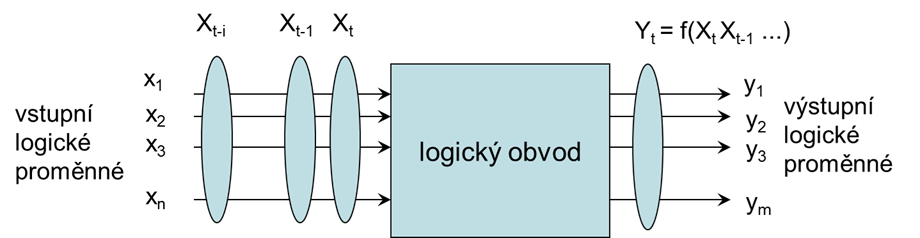
\includegraphics[scale=0.5]{fig/sekvencni_model.png}
		\end{center}
	
		\begin{itemize}
			\item vstupy a výstupy nabývají pouze logických hodnot, tj. 0 1,
			\item stav výstupu závisí navíc na časové posloupnosti (sekvenci) vstupů,
			\item obvod obsahuje paměť pro uchování stavu.

		\end{itemize}
	
	\end{frame}
	
% =====================================================================================================================
	\begin{frame}
    \frametitle{Huffmanův model automatu}
		
		\begin{center}
			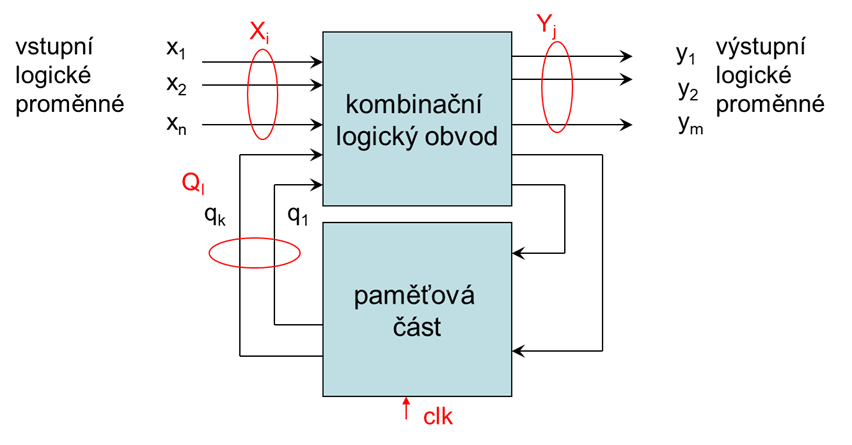
\includegraphics[scale=0.5]{fig/huffmanuv_model.png}
		\end{center}

	\end{frame}

% =====================================================================================================================
	\begin{frame}
    \frametitle{Popis sekvenčního logického obvodu}
	
		\begin{itemize}
			\item Proměnné systému:
			
			\begin{itemize}
				\item[$X$] ... vstupní proměnné,
				\item[$Q$] ... stavové proměnné, musí existovat počáteční hodnota,
				\item[$Y$] ... výstupní proměnné.
			\end{itemize}
			
			\vspace{3mm}
			\item Stavově přechodová funkce:
			\begin{center}
				$\delta : \;f(Q_{n-1},X_n) = Q_{n}$
			\end{center}
			
			\vspace{3mm}
			\item Výstupní funkce:
			
			\begin{itemize}
				\item typ \textbf{Mealy}:
					\begin{center}
						$\lambda : \;f(Q_{n-1},X_n) = Y_{n}$
					\end{center}
				\item typ \textbf{Moore}:
					\begin{center}
						$\lambda : \;f(Q_{n-1}) = Y_{n}$
					\end{center}
			\end{itemize}
			
		\end{itemize}
	
	\end{frame}
	
% =====================================================================================================================
	\begin{frame}
    \frametitle{Model Mealy x Moore}
	
		\textbf{Mealy} - výstup je definován jak stavem tak vstupem:
		\begin{center}
			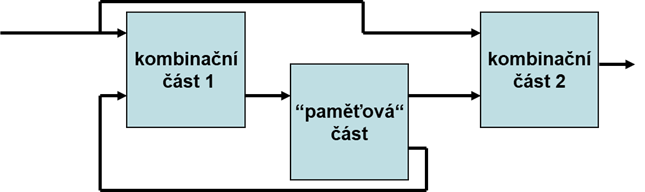
\includegraphics[scale=0.5]{fig/mealy_model.png}
		\end{center}
		
		\vspace{3mm}
		\textbf{Moore} - výstup je definován jen stavem:
		\begin{center}
			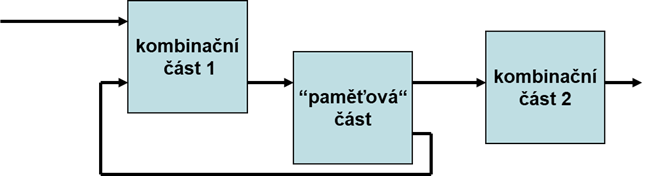
\includegraphics[scale=0.5]{fig/moore_model.png}
		\end{center}
	
	\end{frame}

% =====================================================================================================================
	\begin{frame}
    \frametitle{Popis diagramem - Mealy}
		
		\begin{minipage}[t][\textheight][t]{0.45\textwidth}
		\small
		\begin{itemize}
			\item Uzly = \textbf{stavy},
			\item spojnice = \textbf{vstup / výstupu}.
		\end{itemize}
		
			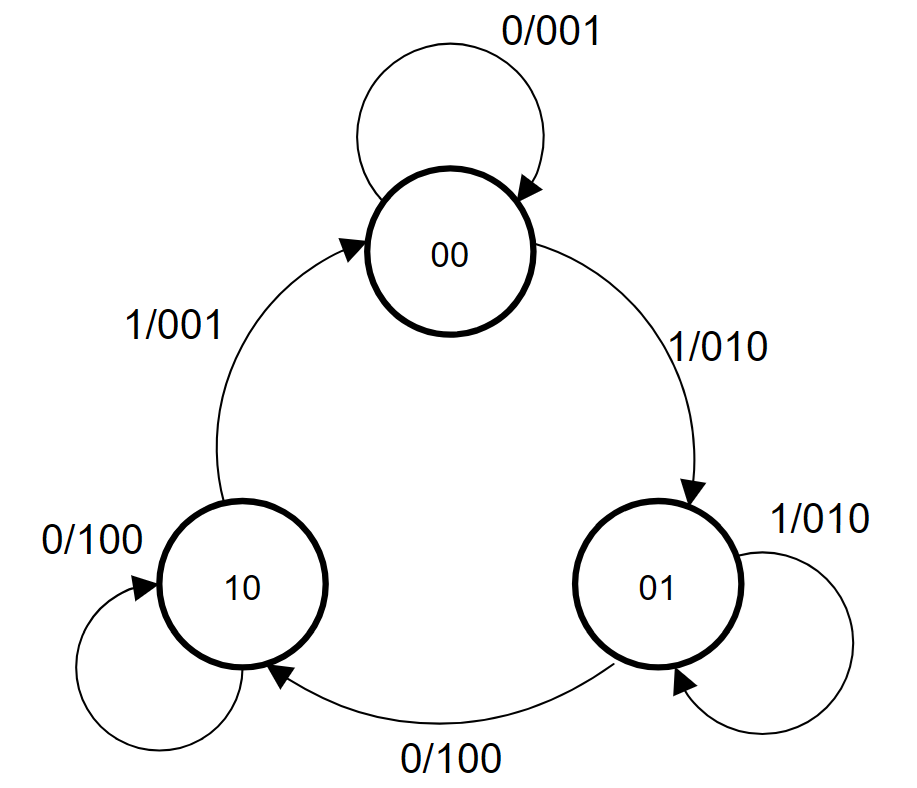
\includegraphics[width=\textwidth]{fig/mealy_diagram.png}

		\end{minipage}
		\begin{minipage}[t][\textheight][t]{0.45\textwidth}
			\vspace{-0.7\baselineskip}
			\begin{center}
				\begin{tabular}{ c c | c }
					$X$ & $Q_{n-1}$ & $Q_n$ \\
					\hline
					0 & 00 & 00 \\
					1 & 00 & 01 \\
					0 & 01 & 10 \\
					1 & 01 & 01 \\
					0 & 10 & 10 \\
					1 & 10 & 00 \\
				\end{tabular}
			\end{center}
			
			\begin{center}
				\begin{tabular}{ c c | c }
					$X$ & $Q_{n-1}$ & $Y_n$ \\
					\hline
					0 & 00 & 001 \\
					1 & 00 & 010 \\
					0 & 01 & 100 \\
					1 & 01 & 010 \\
					0 & 10 & 100 \\
					1 & 10 & 001 \\
				\end{tabular}
			\end{center}

		\end{minipage}
		
	\end{frame}
	
% =====================================================================================================================
	\begin{frame}
    \frametitle{Popis diagramem - Moore}
		
		\begin{minipage}[t][\textheight][t]{0.45\textwidth}
		\small
		\begin{itemize}
			\item Uzly = \textbf{stav / výstup},
			\item spojnice =\textbf{vstupy}.
		\end{itemize}
		
			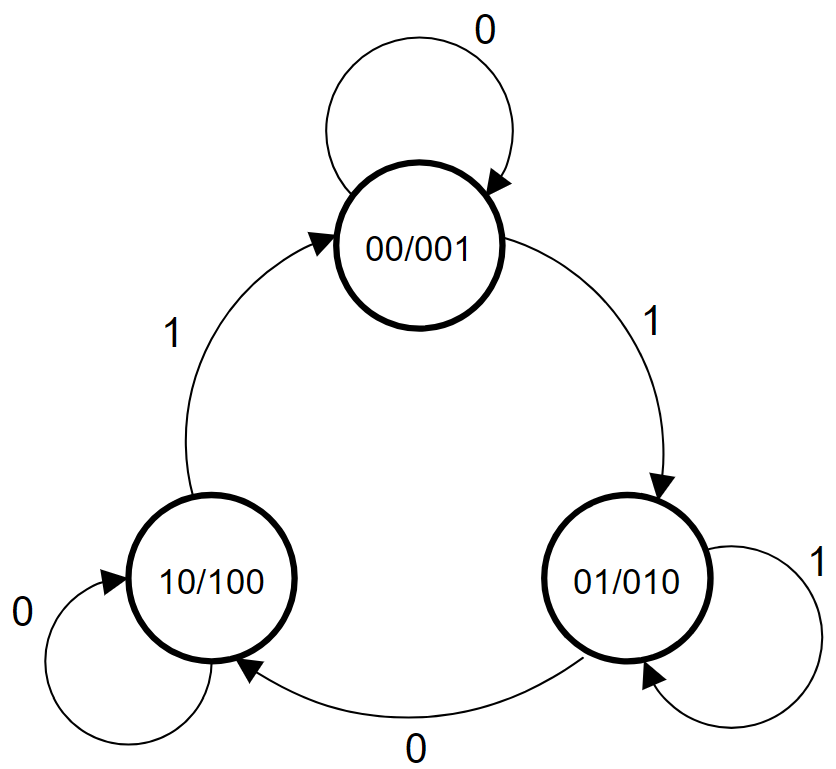
\includegraphics[width=0.9\textwidth]{fig/moore_diagram.png}

		\end{minipage}
		\begin{minipage}[t][\textheight][t]{0.45\textwidth}
			\vspace{-0.7\baselineskip}
			\begin{center}
      $\delta:$
				\begin{tabular}{ c c | c }
					$X$ & $Q_{n-1}$ & $Q_n$ \\
					\hline
					0 & 00 & 00 \\
					1 & 00 & 01 \\
					0 & 01 & 10 \\
					1 & 01 & 01 \\
					0 & 10 & 10 \\
					1 & 10 & 00 \\
				\end{tabular}
			\end{center}
			
			\begin{center}
      $\lambda:$
				\begin{tabular}{ c | c }
					$Q_{n-1}$ & $Y_n$ \\
					\hline
					00 & 001 \\
					01 & 100 \\
					10 & 001 \\
				\end{tabular}
			\end{center}

		\end{minipage}
		
	\end{frame}